\documentclass[12pts]{article}

\usepackage[margin=1in]{geometry}
\usepackage[usenames, dvipsnames]{color}
\usepackage{setspace}
\usepackage{graphicx}
\doublespacing
\usepackage{fancyvrb}
\usepackage{varwidth}
\usepackage{verbatim}
\usepackage{multicol}
\usepackage{enumitem}
\usepackage{float}
\usepackage{fancyhdr}
\usepackage{parskip}    % This packages sets the spacing between two paragraphsc   
\usepackage{hyperref}              
\setlength{\parskip}{.5\baselineskip}   % Define spacing between two paragraphs

\setlength{\parindent}{0pt}
\setlength{\columnseprule}{0pt}

% Title Page
\title{DIME DYNAMIC DOCUMENTS TRAINING \\ Exercise 2}
\author{Luiza Andrade \& Mrijan Rimal} 
\date{\today}

\makeatother


\begin{document}
	
	
	\makeatletter
	\begin{titlepage}
		\begin{center}
			
\includegraphics[width=0.3\linewidth]{../img/i2i.png}\\[10ex]
			{\LARGE \bfseries  \@title }\\[2ex] 
			{\Large  \@author}\\[20ex] 
			{\large \@date}
		\end{center}
	\textcolor{red}{For the most recent version of the file, please check \url{https://github.com/worldbank/DIME-LaTeX-Templates/}}
	\end{titlepage}
	\makeatother
	
	\tableofcontents
	
	\begin{minipage}{\textwidth}
		
	\section*{Introduction}
	Exercise 1 introduced you to the basics of how to import tables and figures to a {\LaTeX} document. This exercise will introduce you to some intermediate topics commonly used to make your document look even more professional.\\
	
	We will also show how {\LaTeX} can be used to create a dynamic document that updates automatically once your output from, for example, Stata or R is updated without any error prone manual copy-and-pasting.
	
	
	
	\section{Exporting tables}
	In this section, you have the option of using the template do file provided in \textcolor{red}{Dynamic-Documentation/Exercises/Stata Export Exercise/Export tables and images.do} to export graphs and figures OR using your own data and generating tables and graphs that can be imported into {\LaTeX}. \\
	
	If you're using the do file provided, change the folder paths in the do file to your directory structure and run the do-file. This will export two tables and two graphs to the Raw folder that will be used in the exercises that follow.  \\
	
	If you would like to work with your own data, please follow the following steps. \\
	
	\begin{enumerate}
		\item Make sure that you export \textbf{two tables} and \textbf{two graphs} using your own data. For help, you can look at the folder called ``Exercise Stata - How to export tables and graph from Stata to LaTeX''.
		\item Make sure that all the exporting is done using Stata do-files, or R scripts so you can easily export them again by just running the code. Towards the end of this exercise we will ask you to make changes to your do-file or R script so if you are using a file from an actual project you may want to make a copy of your do-file or R script that you can use in this exercise.
		\item Open up the \textit{Exercise 2.tex} file and import all the tables and figures you have created in step 1 into your {\LaTeX} document. Sample code to import tables and figures can be found in the templates in the \textbf{DIME Templates} folder.
		\item Make sure you give a caption to your tables. 
	\end{enumerate}
	%KB: why do we ask them to use differnt templates for figures and tables and then in the next section ask them to create one section for tables and one for figures in the same document?
	\end{minipage}
	
	
	\section{Intermediate {\LaTeX} Exercises}
	\subsection{Adding Sections to your document}
	{\LaTeX} automatically formats the document and different section headers and subheaders according to predefined formats. It also allows you to automatically create a \texttt{Table of Contents} based on what has been defined as sections and subsections. 
	
	Sections can be created using \verb|\section{title}| command. {\LaTeX} automatically numbers all the sections in the order you put them. Since you don't manually specify chapter and section numbers, you can cut and paste subsections from the end to the beginning and their numbering will update automatically! 
	
	Similarly, subsections can be created using \verb|\subsection{title}| and sub-sub-sections can be created using \verb|\subsubsection{title}|. The subsections will be numbered on the format 1.1 and the subsubsection will be numbered on the format 1.1.1.
	
	\textcolor{BurntOrange}{\textbf{Task 1:}} Create two different sections in your {\LaTeX} document, one called \emph{Tables} and other called \emph{Figures}.
	
	\textit{Note: Sections and subsections can be created using} \verb|\section*{title}| \textit{if you do not want your sections numbered in the document. However, these sections and subsections will not be shown in the table of contents.}
	
	\subsection{Adding Table of Contents}
	
	After we have set up sections, sub-sections and sub-sub-sections you can easily add a table of contents to your {\LaTeX} document by typing \verb|\tableofcontents| in your document. You can create this anywhere you want, but it is typically created right after \verb|\begin{document}| -- or \verb|\maketitle| if you have a title.  An example is shown below:
	
	\begin{minipage}{\textwidth}
	\begin{Verbatim}[commandchars=+\(\)]
	\documentclass[12pts]{article}
	
	\title{My Awesome Document}
	\author{John Doe}
	
	\begin{document}
	\maketitle
	+color(CornflowerBlue)\tableofcontents
	\newpage
	
	\end{Verbatim}
	
\end{minipage}
	The above {\LaTeX} code is used to generate table of contents below.
	
	\begin{figure}[H]
		\centering
		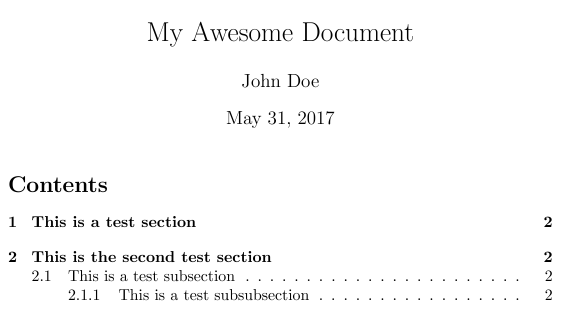
\includegraphics[width=.8\linewidth]{../img/tableofcontents2}
		\caption{Example table of contents generated from our document in Annex 1.}
		\label{fig:tableofcontents}
	\end{figure}

	\textcolor{BurntOrange}{\textbf{Task 2:}} Add a table of contents to the first page of your {\LaTeX} document.
		
	\subsection{Referring to your tables, and figures in a document}
	
	Just like the numbering of section and sub-sections, {\LaTeX} uses a dynamic referencing system for tables and figures etc. In part of your text where you describe tables and figures you are likely to want to refer to them on a format similar to ``\textit{As you can see in figure 2...}". Since the numbering of tables and figures is updated automatically, you need a way for your references in your text to be updated automatically as well.
	
	In {\LaTeX} that is solved by giving tables and graphs a unique name using the \verb|\label{}| command. In the text where you want to reference a figure or a table, you reference the name used in the label and {\LaTeX} will update the numbering for you as your documents grows and changes.
	
	The labels are categorized into the type of item you are referencing, so you label tables and figures slightly differntly. We will show how it is done in the following sub-sections.
	
	\textcolor{BurntOrange}{\textbf{Task 3:}} Below the first figure of your file, write a short paragraph describing it.
	
	\subsubsection{Referring to Figures in a document}
	To refer to figures, we will use the \verb|\label{fig:figurename}| command. Inside the brackets in the \verb|\label{}| command you see two parts seperated by a colon. The first part (\texttt{fig}) indicates that this is a figure that we are assigning a label to. The second part (\texttt{figurename}) should be replaced with the unique name you want to use to refer to this figure.
	
	We must add the \verb|\label{fig:figurename}| line inside the figure environment in our codes, and below the caption. Otherwise, it will be not be displayed correctly. Here's an example:
	
	\begin{Verbatim}[commandchars=+\(\)]
	\begin{figure}[H]
		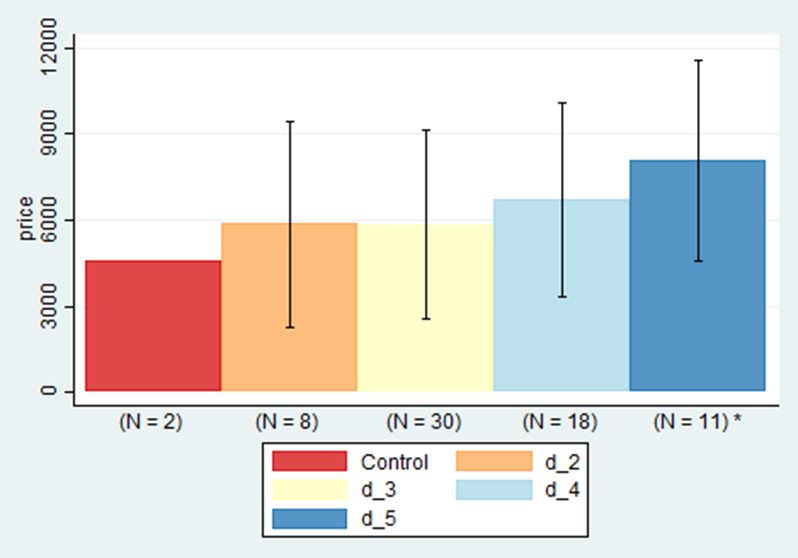
\includegraphics[width=\textwidth]{../Raw/iegraph.png}
		\caption{Add figure title here}
		+color(CornflowerBlue)\label{fig:iegraph}
	\end{figure}
	\end{Verbatim}
	
	Now you can type \verb|\ref{fig:iegraph}| to refer to this figure and it will be automaticallyupdated using the correct number in the document. In our example, if the \texttt{iegraph} figure is the fourth one in the document, \verb|As you can see in figure \ref{fig:iegraph}| will be displayed as \emph{As you can see in figure 4} in the document. 
	
	\textcolor{BurntOrange}{\textbf{Task 4:}} Edit the paragraph you wrote below figure 1 to include a dynamic referrence to it. Use \emph{Build \& View} to check that it works.
	
	\textcolor{BurntOrange}{\textbf{Task 5:}} Change the order of the two figures in your document and make what used to be the second figure the first one. Use \emph{Build \& View} to update your PDF and make sure that the figure reference was updated.
	
	\subsubsection{Referring to Tables in a document}
	
	Similarly for tables, we can also refer to them anywhere in the document using the same method. To refer to tables, we will use \verb|\label{tab:tablename}| command inside the table environment and below the caption, as in the example below. 
	
	\begin{Verbatim}[commandchars=+\(\)]
	\begin{table}[H]
		\caption{Add a title to this table}
		{
\def\sym#1{\ifmmode^{#1}\else\(^{#1}\)\fi}
\begin{tabular}{l*{4}{c}}
\hline\hline
          &\multicolumn{1}{c}{Group 1}&\multicolumn{1}{c}{Group 2}&\multicolumn{1}{c}{Group 3}&\multicolumn{1}{c}{Group 4}\\
\hline
Control   &       203         &       945         &        700         &        200         \\
Treatment &       151         &       952         &        952         &        148         \\
\hline
Total     &       354         &       1897         &       1652         &       348         \\
\hline\hline
\end{tabular}
}

		+color(CornflowerBlue)\label{tab:samplesize}
	\end{table}
	\end{Verbatim}
	
	\subsection{Text Formatting}
	
	Now that you have created sections in your document, and added text, you might want to change some of the formatting of your text. In {\LaTeX} you format your text using packages and code. We will here include a few topics.
	
	\subsubsection{Bold, italic and underlined}
	
	You can make part of your text bold using \verb|\textbf{text}|. To 	underline part of your text, use \verb|\underline{text}|. To make part of your text italic use \verb|\textit{text}|. Here's how it looks:
	
	\begin{center}
		\begin{multicols}{2}
			\verb|\textbf{This is a bold text.}| \\
			\verb|\underline{This is an underlined text.}| \\
			\verb|\textit{This is an italic text.}| \\
			
			\columnbreak
			
			\textbf{This is a bold text.} \\
			\underline{This is an underlined text.} \\
			\textit{This is an italic text.}
		\end{multicols}
	\end{center}
	
	\textcolor{BurntOrange}{\textbf{Task 6:}} Choose some words in your text paragraph to be turned into bold, italic and underline. If you're using TeXStudio, you can use the shortcuts \texttt{CTRL+B} for bold and \texttt{CTRL+I} for italic.
	
	\subsubsection{Text color}
	Font color can be changed using \verb|\textcolor{color}{text}|. You can find a list of color options in the \href{https://en.wikibooks.org/wiki/LaTeX/Colors}{{\LaTeX} WikiBook}, but here are a few examples:

% TO-DO: say that you need to type usepackage in the preamble
	
	\clearpage
	\begin{center}
		\begin{multicols}{2}
			\verb|\textcolor{red}{This is a read text.}| \\
			\verb|\textcolor{Gray}{This is a gray text.}| \\
			\verb|\textcolor{Cyan}{This is a Cyan text.}| \\
			\verb|\textcolor{RoyalPurple}{This is a RoyalPurple text.}|
			
			\columnbreak
			
			\textcolor{red}{This is a read text.} \\
			\textcolor{Gray}{This is a gray text.} \\
			\textcolor{Cyan}{This is a Cyan text.} \\
			\textcolor{RoyalPurple}{This is a RoyalPurple text.}
		\end{multicols}
	\end{center}
	
	\textcolor{BurntOrange}{\textbf{Task 7:}} Change the color of a sentence in your paragraph. Try combining \verb|\textcolor| with \verb|textbf|.
		
	
	\subsection{Making a Dynamic Document}
	
	Here, we will produce a dynamic document. Please only do this do \textbf{if} you have completed all tasks up to \texttt{Part 2.5} of this exercise document and generated a document. This part will show you how easily {\LaTeX} is updating your formatted documents without having to make any manual changes or manually copy and paste any files, code or results.
	
	\begin{enumerate}
		\item Make sure that the you have generated a PDF document by compiling the your {\LaTeX} code. Now copy the PDF created to a separate location from where {\LaTeX} is exporting it. You will only need this second copy of your PDF document temporarily, so you can copy it to your desktop for example. 
		\item Make a significant change to your dataset by, for example, dropping a large subset of your data set. You want to make such a large change to your dataset that when you re-run your do-file or your R script, your outputs should look very different.
		
		If you are using the Stata do-file template provided in the Dynamic Documentation Folder, then only keep observations with population growth more than 0. This can be done by using the Stata codes \texttt{drop if popgrowth < 0}. 
		\item Rerun the do-file or R script you used to generate the tables and files you imported to {\LaTeX} in this exercise. Make sure to not change any file paths to where your tables and graphs were exported. You want your own tables and graphs to be replaced and overwritten.
		\item Now, go back to the {\LaTeX} code where you have imported the tables and graphs for this exercise and generate the pdf document again. Press \textit{Build and Compile} under the \textit{Tools}.
		\item Now if you compare the PDF file you have just generated with you new data with the one you saved in a different folder in the beginning of this section, you will find that the tables have updated automatically without you having to do any manual edits. 
	\end{enumerate}
	
	In this part you updated your tables and figures in the final document without having to copy any results or files manually. Such manual updates are by far the most common reason for errors while generating and sharing research results. This is the most important reason why we at DIME are promoting {\LaTeX}, as manual errors cause us to lose a lot of time and in the worst case leads to mistakes in results that are published.
	
	\section{Additional {\LaTeX} features}
	
	\subsection{Rotating a table}
	
	Sometimes the tables are very wide and need to be in landscape format. This can be adjusted using the \texttt{adjustbox} package which we have been using for importing tables. To rotate the table to landscape, we can use the \texttt{adjustbox} feature with the \texttt{angle = 90} option as shown in blue in the code below.
	
	\begin{minipage}{\textwidth}
		\begin{Verbatim}[commandchars=+\(\)]
		\begin{table}[H]
			\caption{Add table title}
			+color(CornflowerBlue)\begin{adjustbox}{angle = 90} 
				{
\def\sym#1{\ifmmode^{#1}\else\(^{#1}\)\fi}
\begin{tabular}{l*{4}{c}}
\hline\hline
          &\multicolumn{1}{c}{Group 1}&\multicolumn{1}{c}{Group 2}&\multicolumn{1}{c}{Group 3}&\multicolumn{1}{c}{Group 4}\\
\hline
Control   &       203         &       945         &        700         &        200         \\
Treatment &       151         &       952         &        952         &        148         \\
\hline
Total     &       354         &       1897         &       1652         &       348         \\
\hline\hline
\end{tabular}
}

			+color(CornflowerBlue)\end{adjustbox}
			\label{tab:samplesize}
		\end{table}
		\end{Verbatim}
	\end{minipage}
	
	This will rotate the table to the specified degree in the final document. 
	
	\subsection{Two tables side-by-side}

	If you want to display two tables next to each other you can create a one-row table where you put each table in a cell each. Note that this is not making the two tables one table, it just neatly puts two tables next to each other. Since it is still two separate tables it only looks good if the two tables are on similar format. For example, if the same table is generated from two subset (male/female, control/treatment etc.) of data set. If you include notes in the .tex files imported in \verb|\input{}| then neither of those notes will be for the same table, instead put the note in the one-row table like in the example below.
	
\begin{minipage}{\textwidth}
	\begin{Verbatim}[commandchars=+\(\)]
\begin{table}[H]
	\centering
	\begin{tabular}{cc}
		\input{"../Output/Raw/tab1_female.tex"}
		&
		\input{"../Output/Raw/tab1_male.tex"}
		\\
		\multicolumn{2}{l}{\footnotesize \textit{Note:} This is a common note.}
	\end{tabular}
\end{table}
	\end{Verbatim}
\end{minipage} 	
	
	
	\subsection{Creating items (bullet points and numbered lists)}
	
	As you have probably noticed in this document, it is also possible to make lists. The \texttt{enumerate} environment created numbered lists, while the \texttt{itemize} environment only creates items.
	
	To make a list, you must first create the environment by typing \verb|\begin{itemize}| and \verb|\end{itemize}|, then type \verb|\item| before each of the items in your list, as shown below:
	
	\begin{multicols}{2}
		\begin{Verbatim}
		Here's a numbered list:
		\begin{enumerate}
		\item Item one
		\item Item two
		\item Item three
		\end{enumerate}
		\end{Verbatim}
		
		\columnbreak	
		
		Here's a numbered list:
		\begin{enumerate}
			\item Item one
			\item Item two
			\item Item three
		\end{enumerate}
	\end{multicols}
	
	\begin{multicols}{2}
		\begin{Verbatim}
		Here's an unnumbered list:
		\begin{itemize}
		\item Item one
		\item Item two
		\item Item three
		\end{itemize}
		\end{Verbatim}
		
		\columnbreak	
		
		Here's an unnumbered list:
		\begin{itemize}
			\item Item one
			\item Item two
			\item Item three
		\end{itemize}
	\end{multicols}
	
\end{document}   